\chapter{Конструкторская часть}

В данном разделе будут представлены схемы последовательного и параллельного вариантов алгоритма Флойда. Будут описаны типы и структуры данных, используемые для реализации, а также структура разрабатываемого программного обеспечения. Кроме того, будут выделены классы эквивалентности для тестирования.

\section{Разработка алгоритмов}

На рисунке \ref{img:floyd} представлена схема последовательного алгоритма Флойда, на рисунке \ref{img:parallel} - параллельного. Схема алгоритма нахождения крайтчайшего расстояния между двумя вершинами показана на рисунке \ref{img:min}. Схема организации многопоточности представлена на рисунке \ref{img:threads}.

\begin{figure}[H]
	\begin{center}
		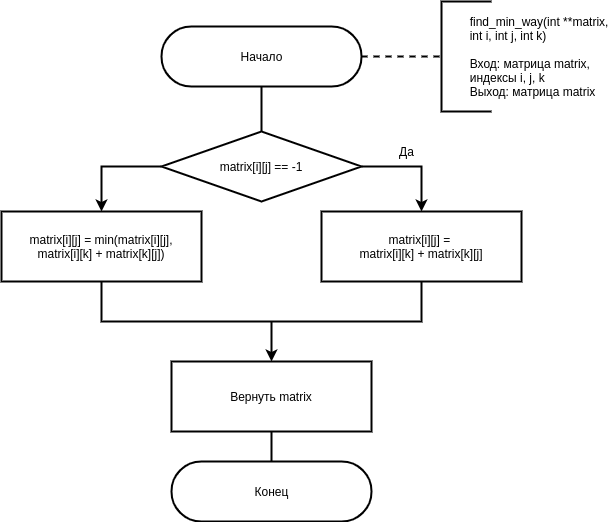
\includegraphics[scale=0.6]{img/min.png}
	\end{center}
	\captionsetup{justification=centering}
	\caption{Алгоритм нахождения кратчайшего пути между двумя вершинами}
	\label{img:min}
\end{figure}

\begin{figure}[H]
	\begin{center}
		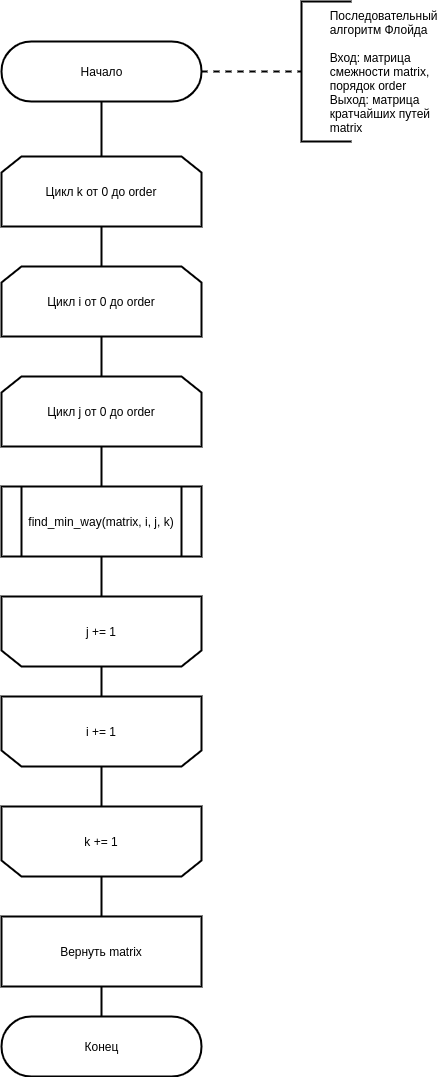
\includegraphics[scale=0.6]{img/floyd.png}
	\end{center}
	\captionsetup{justification=centering}
	\caption{Последовательный алгоритм Флойда}
	\label{img:floyd}
\end{figure}

\begin{figure}[H]
	\begin{center}
		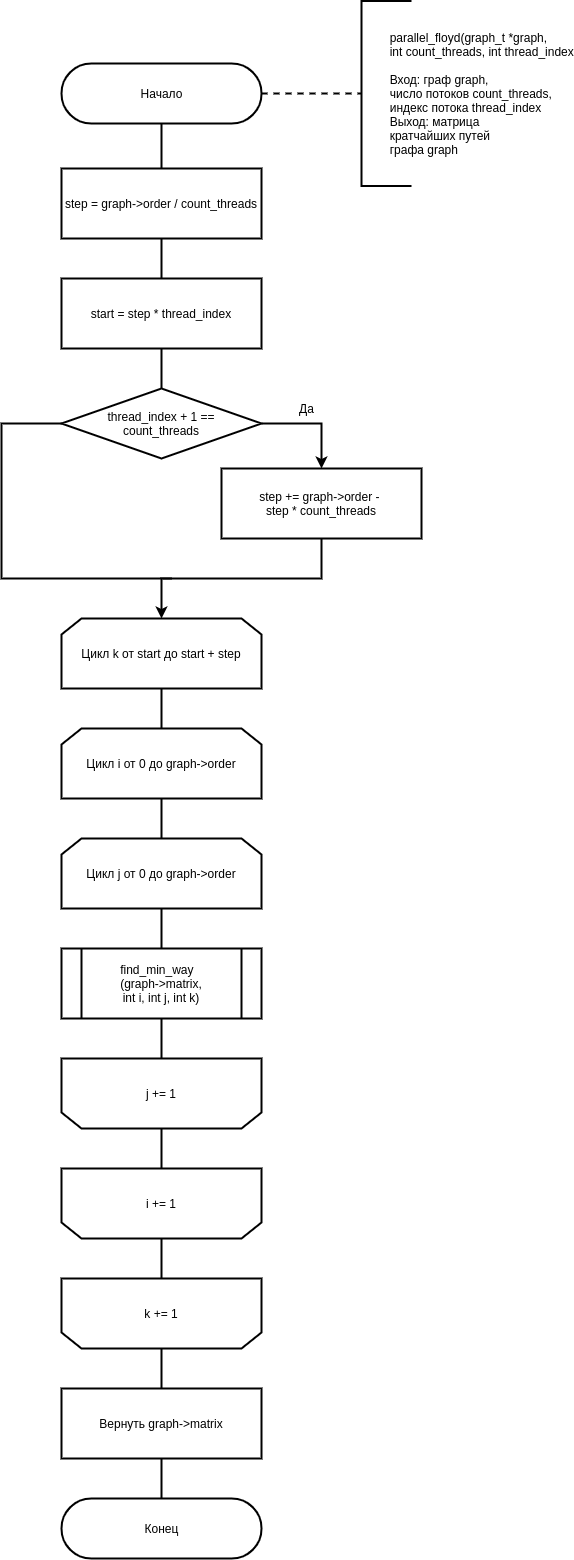
\includegraphics[scale=0.4]{img/parallel.png}
	\end{center}
	\captionsetup{justification=centering}
	\caption{Параллельный алгоритм Флойда}
	\label{img:parallel}
\end{figure}

\begin{figure}[H]
	\begin{center}
		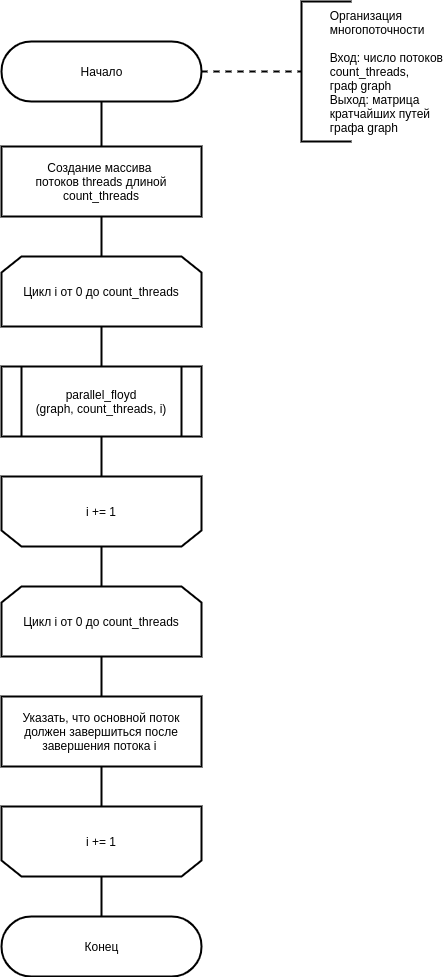
\includegraphics[scale=0.6]{img/threads.png}
	\end{center}
	\captionsetup{justification=centering}
	\caption{Организация многопоточности}
	\label{img:threads}
\end{figure}

\section{Описание используемых типов и структур данных}

Для реализации многопоточности будет использован тип данных $int$ - для числа потоков.

Для представления графа будет использована структура данных $graph_t$, которая имеет следующие поля:

\begin{itemize}
	\item $order$ - число типа $int$, которое задает порядок графа;
	\item $matrix$ типа $int **$  - массив указателей на указатели на целые числа, который задает матрицу смежности.
\end{itemize}

\section{Структура разрабатываемого ПО}

При реализации разрабатываемого программного обеспечения будет использоваться метод структурного программирования. Для взаимодействия с пользователем в функции $int main(void)$ будет реализовано меню, при помощи которого будут вызываться последовательный и параллельный методы нахождения матрицы кратчайших путей в графе и функции сравнительного анализа. Для работы с графом будут разработаны следущие функции, входным параметром которых является указатель на структуру графа:

\begin{itemize}
	\item процедура инициализации графа; 
	\item создание графа со случайными весами ребер, выходным параметром функции является сгенерированная матрица смежности;
	\item ввод графа, выходным параметром является введенная матрица смежности;
	\item процедура вывода графа;
	\item процедура освобождения памяти из-под матрицы смежности;
	\item функции поиска кратчайших путей между двумя любыми вершинами в графе для каждого алгоритма(последовательного и параллельного), у которых на выходе - матрица кратчайших расстояний между любыми двумя вершинами в графе. 
\end{itemize}

Для сравнительного анализа будут реализованы:

\begin{itemize}
	\item функции замеров времени, входными параметрами которых являются граф и число потоков, выходным парметром - массив временных значений;
	\item функция графического представления замеров времени, у которой на входе - массив временных значений, на выходе - его графическое представление.
\end{itemize}

\section{Классы эквивалентности при тестировании}

Для тестирования разрабатываемой программы будут выделены следующие классы эквивалентности:

\begin{itemize}
	\item некорректный порядок графа (меньше 2);
	\item некорректный вес графа (не число или число, меньшее -1);
	\item некорректный ввод числа потоков (меньше 1);
	\item корректный ввод всех параметров.
\end{itemize}

\section{Вывод}

Были представлены схемы поиска кратчайших расстояний между двумя любыми вершинами в графе. Были указаны типы и структуры данных, используемые для реализации, и описана структура разрабатываемого программного обеспечения. Также были выделены классы эквивалентности для тестирования ПО.
